\documentclass[10pt,final,journal]{IEEEtran}
\usepackage{xcolor} % Allows to make use and define many colors.
\usepackage[numbers]{natbib}
\usepackage{graphicx}
\usepackage{lipsum}

\newcommand{\todo}[1]{\color{red}\_ToDo: #1 \color{black}}
\graphicspath{{./img/}}
\title{Room localisation in the Museum of Fine Arts in Ghent using painting recognition}
\author{Bert De Saffel, Timothy Thiecke}
\begin{document}
	\maketitle
	\begin{abstract}
		This paper describes our method to localise a painting on a ground plan based on The Musem of Fine Arts in Ghent. 
	\end{abstract}


	\section{Introduction}
	This paper introduces a framework for rapid painting detection.
	\todo{What makes this work useful?}
	
	\todo{Why should someone spend time to read this paper}
	
	\todo{clarification of title and context}
	
	\todo{which problem has been solved}
	
	\todo{overview of related work}
	
	\todo{benefits and shortcomings of related work}
	
	\todo{overview of your own contributions}
	This paper contains $x$ contributions:
	\todo{overview of results}
	
	\todo{why these results are useful}
	
	\todo{overview of structure of the paper}
	In section 2 ...
	The Museum of Fine Arts in Ghent houses a large collection of mostly Flemish art such as paintings and sculptures. The museum allows its customers to take photographs or videos of most art pieces for own usage. 
	
	Based on a frame from a ca which contains a painting, 
	
	Figure \ref{fig:groundplan_msk} shows the ground plan that is used to mark the correct room
	
	\begin{figure}
		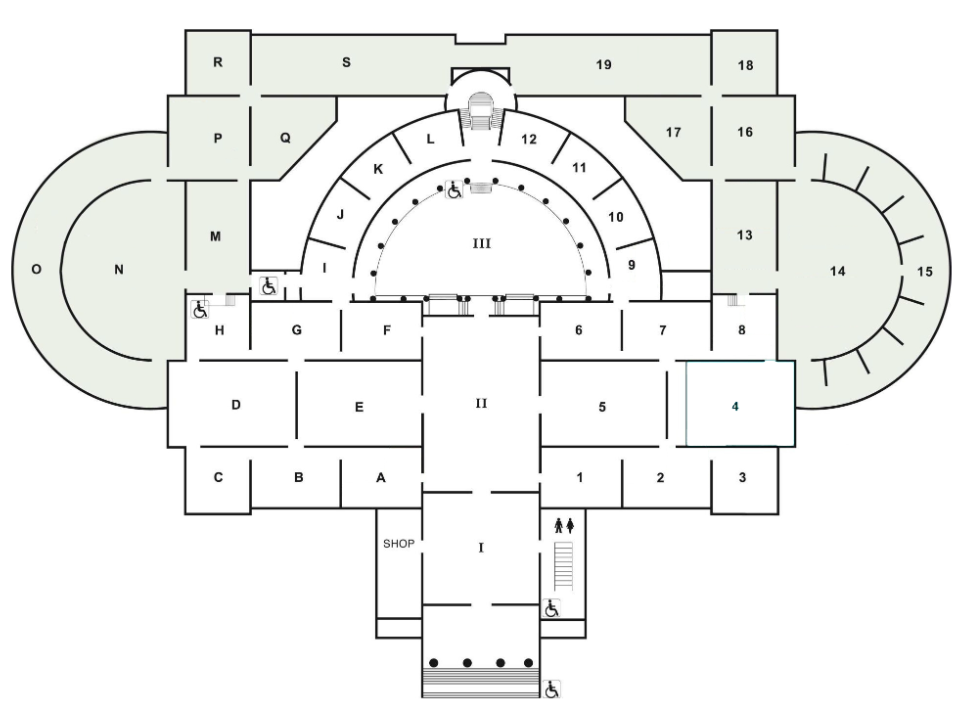
\includegraphics[width=\linewidth]{groundplan_msk}
		\caption{A ground plan of The Museum of Fine Arts, Ghent. }
		\label{fig:groundplan_msk}
	\end{figure}

	\section{Painting Detection}
	\todo{ook dingen uitleggen die niet werkte}
	\begin{itemize}
		\item \todo{vanishing points}
		\item \todo{hough transformatie}
		\item \todo{lijn intersectie}
		\item \todo{gabor filter}
		\item \todo{local binary patterns}
	\end{itemize}

	\todo{gebruik ook afbeeldingen}
	\lipsum[6]
	
	\subsection{Painting Segmentation}
	Before a painting can be matched against the database it must first be recognized in an arbitrary frame. 
	
	\subsection{Feature detection}
	\lipsum[12-15]
	\section{Results}
	\todo{qualitative as well as quantitative}
	
	\todo{quantitative: graphs, tables, roc-curves, f1-scores, ...}
	
	\todo{qualititative: technisch, show where and why the method succeeds or fails, pictures of easy and difficulty cases}
	\lipsum[16-18]
	\section{Conclusion}
	\todo{overview of the most important contributions and the results, without introducing anything new}
	
	\todo{after the reader has read the paper, the reader can look at the contributions and results from a different viewpoint}
	
	\todo{statements can be made more explicit}
	
	\todo{eventueel future work}
	\lipsum[19]

	\bibliographystyle{IEEEtran}
	\bibliography{IEEEabrv,library}
\end{document}